\documentclass{beamer}
\documentclass{abntex}

% Pacotes
\usepackage[utf8]{inputenc}

%% Configurações do Template, Imagem de Fundo[../template7.jpg], e Tema de apresentação[Madrid]
\usebackgroundtemplate{
  \includegraphics[width=\paperwidth,
  height=\paperheight]{../template7.jpg}
}
\usetheme{Madrid}

%% Mudança de dimenções da apresentação
\mode<presentation>


%% Produção da Capa de Aprensentação
\title[Relatórios]{\Huge{Produção de Relatórios, Pacote ABNTeX}}
\author[Branquinho]{Pedro Gomes Branquinho \\
  \text{\scriptsize{pedro.branquinho@usp.br}}}
\date[ABNTeX]{\scriptsize{Mini-curso de \LaTeX \\ Universidade de São Paulo - DEMAR}}


%% Início do documento
\begin{document}

%%Para a Capa, usaremos uma imagem diferente, com o brasão da USP, e logomarca.
{\usebackgroundtemplate{
\includegraphics[width=\paperwidth]{../Imagens/TP.jpg}}
  \begin{frame}
    \titlepage
  \end{frame}
}

%% Notas de versões anteriores
% \begin{frame}
%   \frametitle{Apresentação em \LaTeX}
%   \tableofcontents[pausecontents]
% \end{frame}


%%Início da Apresentacão, o que esperar
\begin{frame}
  \section{Motivações}
  \frametitle{Motivações}

  \begin{enumerate}
  \item<1->{Alto Nível de Produção Texual}
  \item<3->{Auto-produção dos Índices, Indexação}
  \item<2->{Tabelas modelo IBGE}
  \item<4->{Fórmulas Matemáticas}
  \item<6->{Formatação de Figuras - Imagens e Gráficos}
  \item<5->{Referências}
  \end{enumerate}

\end{frame}

\begin{frame}

  \section{Pacote ABNTeX}
  \frametitle{O que é, e como usar o pacote abnTeX}
  \pause
  \setbeamercolor{block title}{fg=white,bg=blue!75!black}
  \begin{block}{ABN\TeX}
    O pacote abnTeX se trata da construção de comandos de formatações
    dentro das normas a ABNT NBR 14724:2011 e a ABNT NBR 6024:2012, as
    quais englobarem os requisitos das demais normas ABNT de produção
    textual. Utilizaremos largamente os \alert{``Modelos Canônicos''} da classe.
  \end{block}
  \pause
 \setbeamercolor{block title}{fg=white,bg=red!75!black}
  \begin{block}{Modelos Canônicos}
  São documentos os quais seguem estritamente as normas ABNT. Porém,
  não necessariamente as especificações de uma intituição. As
  instituições brasileiras adotam particularidades, com pequenas
  variações, em relação aos modelos canônicos.
 \end{block}

%   \begin{example}[Exemplos]
%     \begin{itemize}

%     \item O Emacs, Vim, Atom, Visual Studio, etc. são interfaces gráficas unificadas. O
%       Emacs recebe título de IDE(Integrated Development Environment)

%       \pause

%     \item Jupiterweb, Moodle, Dedalus são sitemas integrados acadêmicos da
%       USP.
%       \pause
%     \item O HTML + CSS são linguagens marcadoras de texto para produção web.
%       \pause
%     \item O \alert{\LaTeX} é uma linguagem - marcadora de texto - para produção de documentos
%       que tenham conteúdo multimídia.
%     \end{itemize}
%   \end{example}
 \end{frame}


 \begin{frame}

  \frametitle{Usando o pacote abnTeX}
  \pause

  No preâmbulo do documento, carregue os pacotes presentes
  no modelo canônico de relatórios técnicos. E, a classe do documento
  como ``abntex2'' - as opções, 12pt, openright, etc. parâmetros configuráveis.

  \pause
  \begin{center}
    \includegraphics<-3>[width=8cm,height=7cm]{../Imagens/A2I1.png}
  \end{center}

\end{frame}

% \begin{frame}
%   \section{Funcionalidades}
%   \frametitle{Sumário, Indíces}
%   Entrar no site github.com, e pesquisar por LaTeX EEL. Baixar o
%   repositório do curso, MC-LaTeX; estudaremos o relatório canônico lá
%   diponível.


% \end{frame}

% \begin{frame}
% %  \section{Funcionalidades}
%   \frametitle{Sumário, Indíces}

%    \begin{itemize}
%   \item{Auto-produção dos Índices, Indexação}
%   \end{itemize}

%   \pause

%  \begin{center}
% %    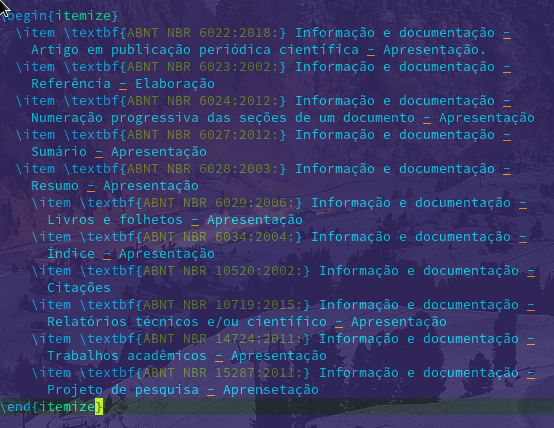
\includegraphics[width=4cm,height=3.5cm]{../Imagens/A2I21.png}
%  %   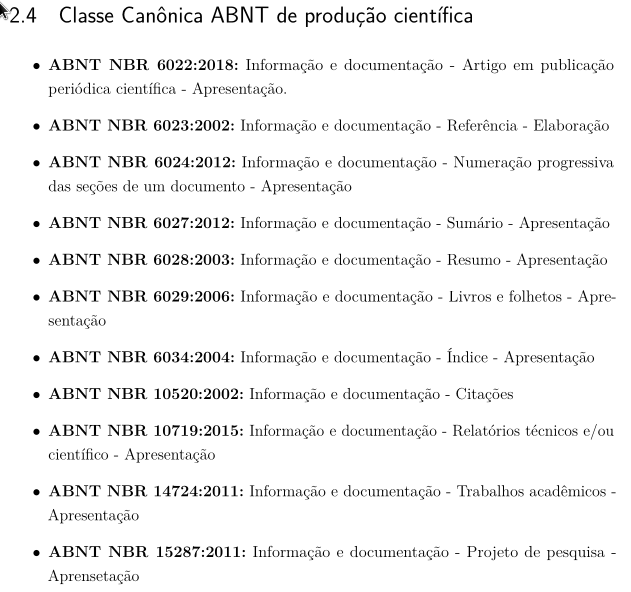
\includegraphics[width=4cm,height=3.5cm]{../Imagens/A2I22.png}
%   \end{center}

%   \pause

%    \begin{center}
%   %  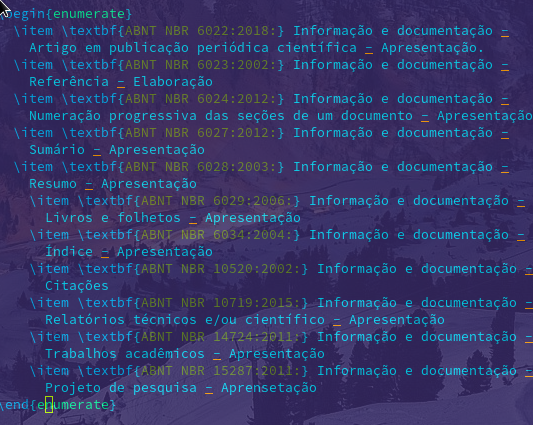
\includegraphics[width=4cm,height=3.5cm]{../Imagens/A2I31.png}
%    % 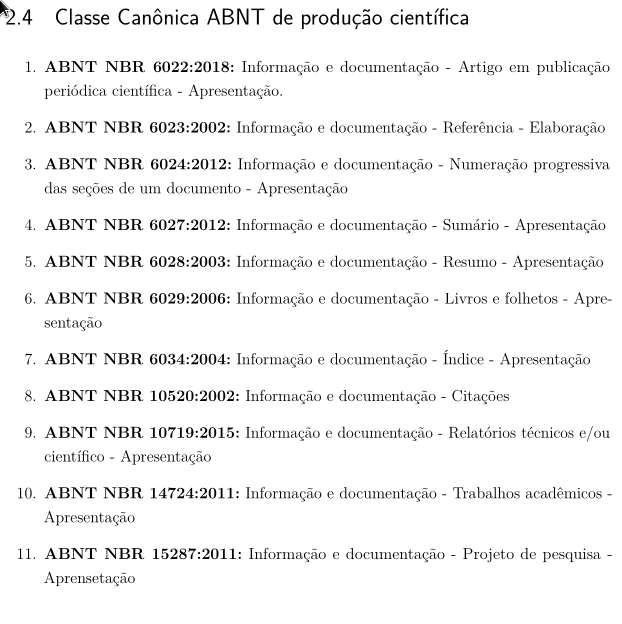
\includegraphics[width=4cm,height=3.5cm]{../Imagens/A2I32.png}
%   \end{center}

% \end{frame}


% \begin{frame}
% \item<4->{Formatação de Figuras - Imagens e Gráficos}
% \end{frame}


\end{document}

%%% Local Variables:

%%% mode: latex
%%% TeX-master: t
%%% End:
